%\documentclass[options]{class}
\documentclass[10pt,journal]{IEEEtran}

%Paquete de Idioma
\usepackage[spanish]{babel}
\usepackage{graphicx}

%Codificación Alfabeto
\usepackage[utf8]{inputenc}
\usepackage{amsmath}
\usepackage{amsfonts}
\usepackage{amssymb}
%\usepackage{amstext} 

%Codificación de Fuente
\usepackage[T1]{fontenc}

%Estilo de Página Numeración superior
%\pagestyle{headings}

%Hiperlinks \href{url}{text}
\usepackage[pdftex]{hyperref}

\usepackage{graphicx}

\begin{document}

%Titulo
\title{Medición del índice de refracción de diversas sustancias}

%Autor
\author{Fernando Dalai Aguilar Sánchez \\ Laboratorio de óptica, ESFM-IPN, Ciudad de México, México \\7 marzo de 2023}


\maketitle{}  

%Resumen
\begin{abstract}
En esta práctica de laboratorio se estudiaron las leyes de reflexión y refracción de la luz. Se realizaron dos experimentos para observar estos fenómenos en diferentes situaciones. En el primer experimento, se utilizó un recipiente semicircular lleno de líquido para observar la refracción de la luz en un alfiler. Se determinaron los ángulos de incidencia y refracción utilizando dos alfileres. En el segundo experimento, se utilizó una placa de vidrio transparente y un láser para observar el fenómeno de reflexión total interna. Se midió el diámetro del círculo blanco y el grosor del vidrio para calcular el índice de refracción del vidrio. 
\end{abstract}  

\section{Introducción}
Ley de reflexión.

Un rayo reflejado permanece en el plano de incidencia (definido como aquel plano que contiene el rayo incidente y la normal a la superficie que separa a los 2 medios) y tiene un ángulo de reflexión igual al de incidencia θi = θi’.

\begin{figure}[!ht]
\begin {center}
\includegraphics[width=0.4\textwidth]{11.png}
\caption{}
\end {center}
\end{figure}

Ley de refracción.

Un rayo refractado permanece en el plano de incidencia y tiene un ángulo
de refracción θt que se relaciona al de incidencia por la ley de Snell:
\begin{align*}
    n_1\sin\theta_1 &= n_2\sin\theta_2 \\
\end{align*} En general: 
\begin{align*}
    n = \frac{c}{v}
\end{align*}
donde $n$ es el coeficiente de refracción, $c$ es la velocidad de la luz en el vacío y $v$ es la velocidad de la luz en el medio en cuestión.


\begin{figure}[!ht]
\begin {center}
\includegraphics[width=0.4\textwidth]{12.png}
\caption{}
\end {center}
\end{figure}


\textbf{Casos particulares:}

\begin{enumerate}
\item Si $n_i = n_t$, no ocurre refracción y el rayo no sufre desviación.
\item Si $n_t > n_i$, entonces $\theta_t < \theta_i$ y el rayo se desvía en una dirección más cercana a la normal a la superficie.
\item Si $n_t > n_i$, entonces $\theta_t > \theta_i$ y el rayo se desvía en una dirección más lejana a la normal a la superficie.
\item Supóngase la situación ii) con el rayo viajando de $n_t$ a $n_i$, suceden entonces las situaciones de propagación ilustradas en la figura 1.
\end{enumerate}

\section{Metodología}


\subsection{Experimento 1.}
Colocamos un alfiler en posición y observamos cómo su patita se refractaba al pasar la luz a travésde un recipiente semicircular lleno de líquido. Para determinar los ángulos de incidencia y de refracción (θi y θt respectivamente), utilizamos dos alfileres como se observa en la figura.


\begin{figure}[!ht]
\begin {center}
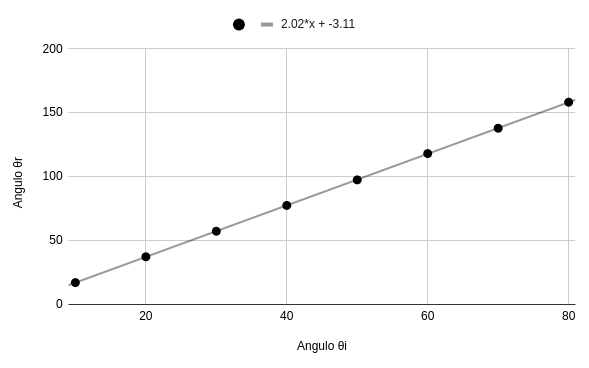
\includegraphics[width=0.4\textwidth]{1.jpg}
\caption{Experimento 1. Primer fluido}
\end {center}
\end{figure}

\begin{figure}[!ht]
\begin {center}
\includegraphics[width=0.4\textwidth]{5.jpg}
\caption{Experimento 1. Segundo fluido}
\end {center}
\end{figure}

\subsection{Experimento 2. Reflexión total interna (Método de Pfund)}
Mediante el uso de una placa de vidrio transparente con fondo blanco y un laser, medimos los círculos en penumbra que se definieron por el fenómeno de reflexión total interna. Medimos el diametro del circulo blanco y el grosor del vidrio para poder calcular el indice de refraccion del vidrio.

\begin{figure}[!ht]
\begin {center}
\includegraphics[width=0.4\textwidth]{7.jpg}
\caption{Experimento 2}
\end {center}
\end{figure}


\section{Resultados}


\subsection{Experimento 1.}


Para el primer fluido se obtuvieron los siguientes datos:
\begin{center}
\begin{tabular}{|c|c|c|}
\hline
N & $\theta$i & $\theta$t \\
\hline
1 & 22 & 34\\
\hline
2 & 3 & 5\\
\hline
3 & 8 & 12.5\\
\hline
4 & 11 & 17\\
\hline
5 & 29 & 47.5\\
\hline
6 & 20 & 29\\
\hline
7 & 2 & 4\\
\hline
8 & 29.5 & 45\\
\hline
\end{tabular}
\end{center}

Al representarlos gráficamente, obtenemos:


\begin{figure}[!ht]
\begin {center}
\includegraphics[width=0.4\textwidth]{9.png}
\caption{Grafica sen($\theta$t) vs sen($\theta$i)}
\end {center}
\end{figure}


Para el segundo fluido se obtuvieron los seguientes datos:

\begin{center}
\begin{tabular}{|c|c|c|}
\hline
N & $\theta$i & $\theta$t \\
\hline
1 & 32 & 50\\
\hline
2 & 9.5 & 15\\
\hline
3 & 15 & 23\\
\hline
4 & 24 & 37\\
\hline
5 & 15.5 & 22\\
\hline
6 & 26 & 40\\
\hline
7 & 25 & 39\\
\hline
8 & 6 & 9.5\\
\hline
\end{tabular}
\end{center}


Al representarlos gráficamente, obtenemos:


\begin{figure}[!ht]
\begin {center}
\includegraphics[width=0.4\textwidth]{10.png}
\caption{Grafica sen($\theta$t) vs sen($\theta$i)}
\end {center}
\end{figure}

.

\subsection{Experimento 2}

Para el vidrio se obtuvieron los siguientes datos: 

\begin{center}
\begin{tabular}{|c|c|c|}
\hline
n &  D(cm) & H(cm)  \\
\hline
1 & 4.82 & 1.52\\
\hline
2 & 4.88 & 1.52\\
\hline
3 & 4.9 & 1.53\\
\hline
4 & 4.95 & 1.53\\
\hline
\end{tabular}
\end{center}

Para el agua se obtuvieron los siguientes datos: 

\begin{center}
\begin{tabular}{|c|c|c|}
\hline
n &  D(cm) & H(cm)  \\
\hline
1 & 7.85 & 1.94\\
\hline
2 & 4.1 & 0.975\\
\hline
3 & 5.6 & 1.28\\
\hline
4 & 9.9 & 2.36\\
\hline
\end{tabular}
\end{center}

\section{Discusión y conclusiones}

\subsection{Experimento 1.}
\item 

 Para el primer fluido, de acuerdo a la función de ajuste que se obtuvo al graficar el seno de los ángulos, podemos obtener el índice de refracción del primer líquido, que es n = 1.438. Proponemos la glicerina como el candidato principal para ser esta sustancia.

Para el segundo fluido, tenemos n = 1.42, por lo que proponemos el aceite vegetal como el candidato para ser esta sustancia.

\item 


\subsection{Experimento 2.}

Para este experimento, nosotros ya conocemos los índices de refracción tanto del agua como del vidrio, los cuales son n = 1.33 y n = 1.45, respectivamente. De acuerdo con los datos obtenidos para el agua, nuestro índice de refracción medido fue n = 1.39, el cual podemos ver que es bastante cercano al original y nos da un error porcentual del 4.5\%. En el caso del vidrio, obtenemos n = 1.58 con un error porcentual del 8.96\%.

\item 






\section{Bibliografía}


Resnick, Halliday y Krane, (2002). Física. VOl I. México. Editorial Cecsa.


Serway, R.A., Jewett, J.W. (2009). "Física: Para ciencia e ingeniería con Física Moderna", 7 Edicion. Vol.2 México. Cengage.


W. Sears, MW Zemansky, HD Young y R. A. Freedman: "Física universitaria", 12 Edición. VOl 2. Addison-Wesley-Longman/Pearson Education.



\end{document}
